\documentclass[11pt, a4paper, hyphens]{article}
\usepackage[a4paper, left=30mm, right=30mm]{geometry} % margin=2.6cm

\usepackage[utf8]{inputenc}  % allow utf-8 input
\usepackage[T1]{fontenc}     % use 8-bit T1 fonts
\usepackage{ebgaramond}

\usepackage{hyperref}         % hyperlinks
\usepackage{url}              % simple URL typesetting
\usepackage{booktabs}         % professional-quality tables
\usepackage{amsfonts}         % blackboard math symbols
\usepackage{nicefrac}         % compact symbols for 1/2, etc.
\usepackage{microtype}        % microtypography
\usepackage{xcolor}           % colors
\usepackage{bbm}
\usepackage{amsthm}
\usepackage{rotating}
\usepackage{pdfpages}

\hypersetup{                 % setup the hyperref package
    colorlinks=true,
    linkcolor=blue,
    filecolor=blue,
    urlcolor=blue,
    citecolor=blue,
    pdftitle={Entitlement Justice and Measures of Algorithmic Fairness},
    pdfauthor={Edward Speer, Llama-2-7b},
    pdfkeywords={entitlement justice, algorithmic fairness, AI ethics},
    bookmarks=true,
}

\usepackage{graphicx} % Required for inserting images
\usepackage[ngerman, english]{babel}
\usepackage[iso, ngerman]{isodate}


\usepackage{bbold}
\usepackage{mathtools}
\usepackage{amsmath} % Required for \DeclareMathOperator
\usepackage{nicefrac}
\usepackage{tikz}
\usepackage{subcaption}
\usepackage{centernot} % for the comparison

%\theoremstyle{definition}
\newtheorem{definition}{Definition}
\newtheorem{theorem}{Theorem}

\usepackage{verbatim}

\RequirePackage[T1]{fontenc} 
\RequirePackage[tt=false, type1=true]{libertine} 
\RequirePackage[varqu]{zi4} 
\RequirePackage[libertine]{newtxmath}

\usepackage[round,comma]{natbib}
\bibliographystyle{plainnat}

\newcommand{\monthyeardate}{\ifcase \month \or January\or February\or March\or %
April\or May \or June\or July\or August\or September\or October\or November\or %
December\fi, \number \year} 

\title{The Role of Large Language Models in Academic Writing}
\author{%
  Edward Speer
  \\
  California Institute of Technology\\
  \texttt{espeer@caltech.edu} \\
}
\date{\monthyeardate}

\begin{document}

\maketitle

\section{Introduction}\label{sec:introduction}

The majority of research journals now provide policies for the use of large
language models (LLMs) as academic writing. The majorioty of these policies are
predicated on the idea that LLMs cannot be the originators of new insights or
novel argumentation, but can function as useful tools in the paper writing
process. In Nature journals, for example, ``Large Language Models do not
satisfy our authorship criteria. Notably, an attribution of authorship carries 
with it accountability for the work, which cannot be effectively applied to
LLMs.'' From the APA, ``The authors are responsible for the accuracy of any
information in their article. Authors must verify any information and citations
provided to them by an AI tool. Authors may use but must disclose AI tools for
specific purposes such as editing.''

The implications of these policies are clear when using LLMs for copy-editing or
or other similar purposes. However, this represents only one mode of interaction
with LLMs. In this paper, we investigate the possibility of interacting with
LLMs in a different mode: as a full intellectual collaborator in the writing
process. To do so, we attempt to undertake the full writing process of an
original philosophical research paper using engaging in full with an LLM as a
coauthor. The purpose of this paper is to assess the success of this endeavor
across several dimensions, including the originality of the ideas presented by
the LLM, the coherence of the argumentation, and the overall quality of the
writing. We also consider the implications of this experiment for the future of
academic writing and the role of LLMs in the research process.

For this project, we chose as the subject of our paper the topic of algorithmic
fairness measures and their connection to the philosophical concept of
distributive justice. Algorithmic fairness measures are a critical component of
the design and deployment of machine learning systems, as they are intended to
ensure that these systems do not discriminate against individuals based on
sensitive attributes. Distributive justice, on the other hand, is a central
concept in political philosophy that concerns the fair distribution of social
goods. Our investigation began from this vague notion of the intersection
between algorithmic fairness measures and distributive justice, and we used the
LLM as a collaborator to help us refine and develop our ideas from this starting
point.

This paper will be structured as follows. In Section~\ref{sec:methods}, we will
present the methods used, including the specific LLM selected for the
investigation and the program used to interact with it. In
Section~\ref{sec:results}, we will present the full text of the paper produced
in collaboration with the LLM. In \ref{sec:analysis}, we will analyze the role
of the LLM throughout 5 stages of the research process: research question
formulation, literature review, argumentation, writing, and revision. Finally,
in Section~\ref{sec:conclusion}, we will conclude with a discussion of the
implications of this experiment for the future of academic writing.

It is critical to aknowledge that the field of machine learning is rapidly
evolving, and the capabilities of LLMs are constantly improving. As such, the
goal of this paper is not to make an assessment of the technological capacity
for LLMs to engage in argumentation, but rather to present insights about how
engaging with LLMs in this way can impact academic writing and the research
process.

\section{Methods}\label{sec:methods}

For this experiment, we selected the Llama-2-7b model developed by Meta AI. The
Llama-2-7b model is a large language model trained on a diverse range of
textual data, including books, articles, and websites. The model is capable of
generating coherent and contextually relevant text across a wide range of
domains. We selected this model for its ability to generate high-quality text
and its general-purpose nature, which makes it suitable for a wide range of
writing tasks, as well as for its open source nature, which reflects our
commitment to transparency and reproducibility.

We engaged with the Llama-2-7b model (henceforth referred to as Llama) using a
web-hosted API called Llama-api (\url{https://www.llama-api.com/}). This API
allows users to pay a per-token fee to interact with the model via an http
request to a designated endpoint. A user sends a prompt to the model, including
context memory built up over the course of the interaction and the limitations
on response tokens, and the model generates a response based on the prompt and
the context memory.

In order to manage the use of Llama, we built a custom chat application in
Python that allowed us to communicate with the model from the command line.
This application has the following features:
\begin{itemize}
    \item \textbf{Chat logging}: User prompts and responses from Llama are
    automatically saved to a log file in markdown format for future analysis.
    \item \textbf{Context Memory Management}: The application allows the user
    to save and use different streams of context memory across different
    sessions with the model. For example, in the beginning of one context, Llama
    is told ``I am a philosopher and computer scientist. You are my co-author.
    We are writing a philosophy paper. We are focused on measures of algorithmic
    fairness and the concept of justice they enforce.'' In another context,
    Llama can be told to act as a reviewer, or to speak in the voice of an
    author encountered in the literature review. These bits of context are saved
    in compressed pickle files and can be loaded into the application at the
    any time during a session.
    \item \textbf{Manual Context Editing}: The application allows the user to
    manually edit the context memory before sending it to Llama. This is useful
    for trimming down the context memory to the most relevant information to
    reduce the cost of the interaction and to focus the model on critical
    information. This feature can also be used to pass entire papers or large
    sections of text to Llama for review or comment.
    \item \textbf{Token Limiting}: The application allows the user to set a
    limit on the number of tokens in the response from Llama. This is useful for
    managing the cost of the interaction with the model.
\end{itemize}
The full source code for the chat application is accessible
from~\ref{sec:appendixI}.

Three main threads of context memory were used to work with Llama in this study.
In the first thread, Llama was presented with the true circumstances of the
experiment: that it was acting as a co-author on a philosophy paper about
algorithmic fairness measures and distributive justice. In the second thread,
Llama was presented with the role of a reviewer of the paper, providing feedback
on the argumentation and writing. In the third thread, Llama was not prompted
with any particular role, but was simply continually asked to explain particular
arguments or concepts from the literature with appropriate citations. Henceforth
we will refer to these roles as the coaauthor, reviewer, and explainer roles. 
Each of these roles was used throughout the research and writing process, with
the exception of the reviewer role which was used only during revision. The full
logs of interactions with the model including which context memory was used in
each interaction are available in~\ref{sec:appendixI}.

\section{Results}\label{sec:results}

What follows is the full text of the paper produced in collaboration with Llama.

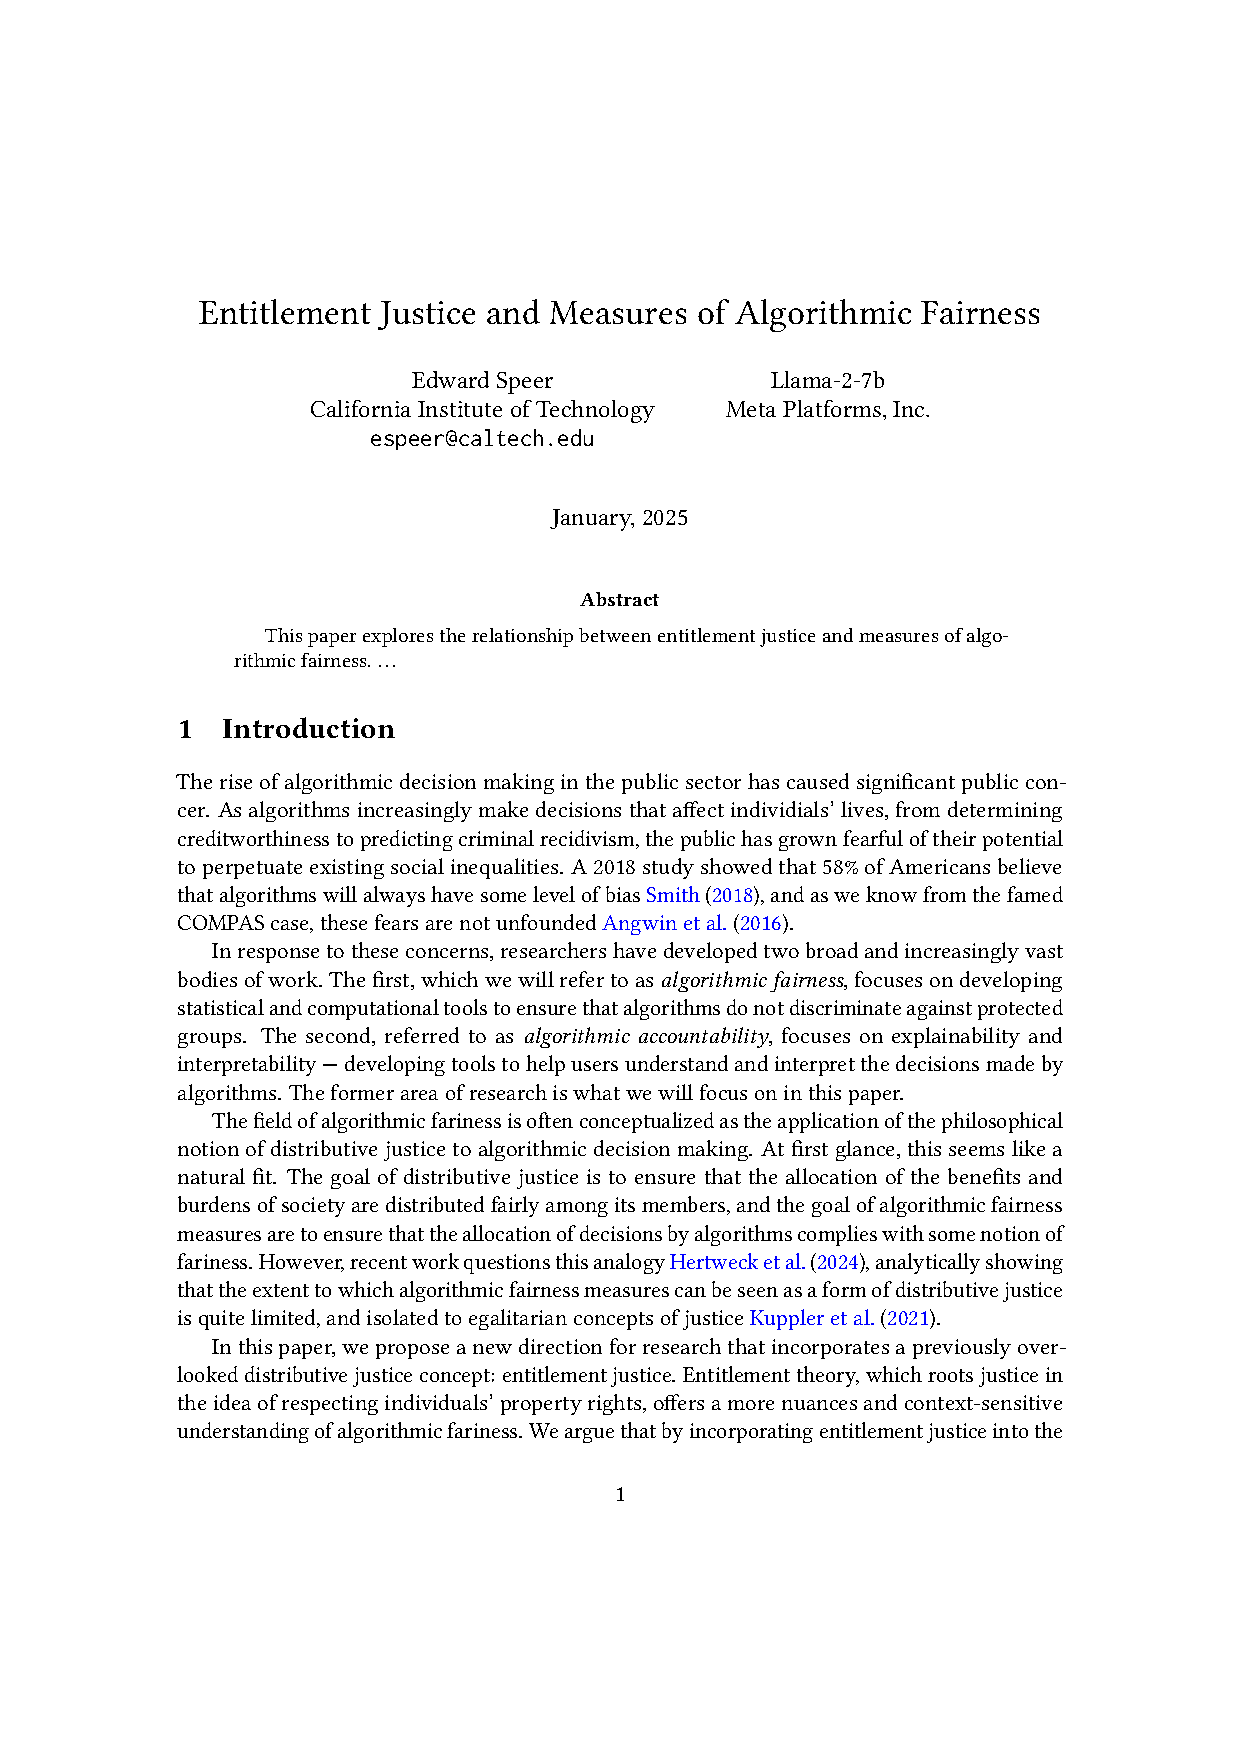
\includepdf[pages=-]{../src/top-level.pdf}

\section{Analysis}\label{sec:analysis}

\section{Conclusion}\label{sec:conclusion}

\section{Appendix I}\label{sec:appendixI}

The full source code for the chat application used in this study as well as all
chat logs are available at the following link: 
\url{https://github.com/Espeer5/paperInAPaper}

% \bibliography{references}
\end{document}